\documentclass{template/openetcs_article}
%\documentclass{article}
%\usepackage[ascii]{inputenc}
%\usepackage[T1]{fontenc}
\usepackage[english]{babel}
\usepackage{amsmath}
\usepackage{amssymb,amsfonts,textcomp}
\usepackage{array}
\usepackage{supertabular}
\usepackage{hhline}
\usepackage{graphicx}
\makeatletter
\newcommand\arraybslash{\let\\\@arraycr}
\makeatother
\setlength\tabcolsep{1mm}
\renewcommand\arraystretch{1.3}
\newcounter{Ilustracin}
\renewcommand\theIlustracin{\arabic{Ilustracin}}
\title{openETCS}

%\setcounter{tocdepth}{3}
\usepackage{float}
\usepackage{hhline}
\usepackage{booktabs}
\usepackage{multirow}
\usepackage{color, colortbl}
\definecolor{myblue}{rgb}{0.6,.6,1}
\definecolor{mydarkblue}{rgb}{0,0,0.5}
\definecolor{mylightblue}{rgb}{0.8,0.8,1}
\usepackage{hyperref}
\hypersetup{colorlinks=true, linkcolor=mydarkblue, urlcolor=mydarkblue}

\usepackage[textwidth=2.7cm,textsize=scriptsize,linecolor=green!40,backgroundcolor=green!40]{todonotes}

\newcounter{mycommentcounter}
\newcommand{\mycomment}[2][]
{
\refstepcounter{mycommentcounter}%
\todo[color={red!100!green!33}]{
\textbf{[\uppercase{#1} \themycommentcounter]:} #2}
}


\usepackage{lipsum,url}
\graphicspath{{./template/}{.}{./images/}}
\begin{document}
\frontmatter
\project{openETCS}

%Please do not change anything above this line
%============================
% The document metadata is defined below

%assign a report number here
\reportnum{OETCS/WP1/Revision and Review processes}

%define your workpackage here
\wp{Work-Package 1: ``Management''}

%set a title here
\title{Project Quality Assurance Plan - Presentation of the Revision and Review Processes}

%set a subtitle here
%\subtitle{A template for short document. Adapted from report template.}

%set the date of the report here
\date{\today}

%define a list of authors and their affiliation here

\author{SQS}

\affiliation{Avda. Zugazarte 8,6\\
  48930 Getxo \\
  Vizcaya, España}


% define the coverart
\coverart[width=350pt]{openETCS_EUPL}

%define the type of report
\reporttype{Description of work}




%=============================
%Do not change the next three lines
\maketitle
\tableofcontents
%\listoffiguresandtables
\newpage
%=============================

% The actual document starts below this line
%=============================


%Start here



%\begin{document}


\section*{Document History}

\begin{flushleft}
%\tablefirsthead{\hline Version & Date & Chapters modified & Reason & Name\\}

\tablehead{\hline \rowcolor{myblue} Version & Date & Chapters modified & Reason & Name\\}

\tabletail{}
\tablelasttail{}
\begin{supertabular}{m{1.1cm}m{1.8cm}m{2cm}m{7cm}m{2cm}lp{6cm}|}
\hline
0.0.1 &
23.05.2013 &
All &
First version &
SQS
\\\hline
0.0.2 &
06.06.2013 &
All &
Second revised version &
SQS
\\
\end{supertabular}
\end{flushleft}

\newpage

\section{Introduction}
Two are the processes defined in OpenETCS to guarantee and maintain the quality of the documents published in the repository:

\begin{itemize}
\item \underline{\textbf{The Revision Process}} -  
Committers and selected Contributors are invited to make contributions to a version of a document before it is published in the Open ETCS repository.
The revision process will be performed:
\begin{itemize}
\item After a first version of the document is created by the authors and when it is plausible significant contributions are still needed to have a complete and publishable document.
\item •	After a major rework of a document or after a review process in which major improvements/comments have been detected.
\end{itemize}
In all cases:
\begin{itemize}
\item The revision process will be carried out in a dedicated Revision Cycle Branch.
\item In case of conflicts, it is the Product Owner who will be responsible for their resolution.
\item The Revision Team is composed of Committers and invited Contributors
\item Contributions/comments are made directly in the document under revision. However, in the case of “Contributors”, the Issue Tracker Tool will be used.
\item The launching, control, notification and clarification processes are managed through the Issue Tracker Tool.
\end{itemize}

\item \underline{\textbf{The Review Process}} - The Open ETCS community is invited to make comments, suggestions or improvements to an already revised document published in the OpenETCS repository. In case major comments are received, a revision process may be launched afterwards.
There are two types of Review Processes:
\begin{itemize}
\item Planned Review Process: It is launched by the product owner; there is a deadline for receiving comments (by default, 2 weeks) from the community and if considered appropriate, there are well identified review objectives and/or guidelines. A Planned Review Process will always be launched after a Revision Process.
\item Open Review Process: At any time, an expert can make comments and suggest improvements to the documents published in the repository. Comments will be assessed by the Product Owner as they are received, and the appropriate actions taken.
\end{itemize}
In both cases:
\begin{itemize}
\item The review process will be performed against documents already revised and therefore published in the repository. Therefore no specific branch for review will be created.
\item All comments will be made and answered using the Issue Tracker tool.
\item The Team of Reviewers is not limited to invited reviewers but to any expert of the Community.
\item The Product Owner will be assisted by a group of selected Key Customers of the document under review when necessary and specifically to resolve conflicts and approve/reject a document and/or launch a new revision process.
\end{itemize}
\end{itemize}

The status (in progress, in revision; revised; in review; active) of each document is maintained in the Wiki page named “Status of documents” of the corresponding project/repository in Github.

\begin{figure}[H]
\centering
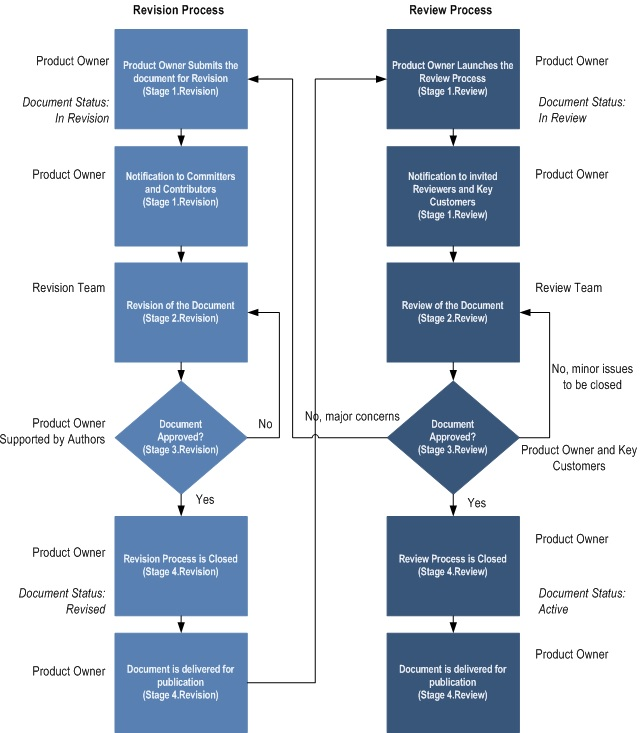
\includegraphics{./figures/RevisionReviewProcess.JPG}
\caption{Revision-Review Processes flow}
\end{figure}

\section{Revision Process}

The revision of the document supports the reworking and/or the incorporation of significant improvements ad contributions to a document. The revision process is controlled by the Product Owner who is supported by the rest of the authors of the document under revision in the process of approving or rejecting changes.

The revision team is composed of the committers of the project the document belongs to and by invited Contributors, if necessary.

Once the document is ready for revision, the product owner launches the process ({\it Stage 1.Revision}). The document status becomes “In revision” and it is uploaded to its corresponding Revision Cycle Branch in the project repository.

The launching and details (dates, scope) of the Revision Process are announced via the Issue Tracker. In this moment, the revision process officially starts.

During the Revision Process ({\it Stage 2.Revision}), committers are expected to make their contributions directly on the document (Latex, ToDoNotes, SmartGit) and contributors via the Issue Tracker.

Interactions between the Revision Team and the Product Owner will be done via the Issue Tracker, so a complete traceability of the process is maintained.

Once the deadline for receiving comments is reached, the Approval Stage starts ({\it Stage 3.Revision}). The Product Owner, supported by the Author(s), revises each of the comments and decides whether approving and implementing or rejecting. 
A final assessment of the comments received will be the basis for the Product Owner to decide whether the document is to be approved or needs further revision (revision process is re-opened).

Once approved, the Closing Stage ({\it Stage 4.Revision}) starts. The Revision Branch is merged into the Master Branch and the document status is set to “Revised”. The Revision Cycle is closed and a Review Process is launched.

\section{Review Process}
The review process implies opening a document for the community to make comments, propose changes and improvements.

As already indicated, any document published in the repository can be reviewed by an expert at any time. Therefore the Review Process can be considered as an Open process. In the case of Open ETCS project, any expert can add a comment to a document in the form of an Issue. The Product Owner is in charge of their analysis and processing.

However, at certain stages of a document life-cycle, it is necessary to plan a review process in which selected reviewers are invited to play an active role. This is identified as a Planned Review Process and described below.

For each document a group of “Key Customers” (users of the document) will be appointed. Key Customers will support the Product Owner in the process of revising, analyzing the relevance and approving/rejecting comments made by the reviewers. 

The Product Owner launches ({\it Stage 1.Review}) the review process (dates, scope) via the Issue Tracker. If necessary, the Project Owner addresses individually the invited reviewers to guarantee their effective participation.

The document is set to status “In review” and the planned review process starts officially.

During the Review Process ({\it Stage 2.Review}), comments are made via the Issue Trackers. Reviewers will be invited to put special attention in labeling the issues properly so they can be easily classified and in revising comments made by other reviewers in order to avoid duplicates.

Interactions (i.e. request of clarifications) between the Revision Team and the Product Owner will be done via the Issue Tracker, so a complete traceability of the process is maintained.

Once the time for comments is over, the Product Owner will go through the comments and select the ones to be implemented and the ones to be rejected or postponed. For this activity and as needed, the Product Owner will have the support of the Key Customers and the Authors.

The Product Owner is responsible for implementing the comments accepted.

Final assessment of the comments and their implementation in the document will be performed by the Product Owner with support of the Key Customers. Conflict resolution will be managed by the Key Customers.

If the document is considered of sufficient quality, the review process will be closed ({\it Stage 4.Review}). Otherwise, further improvements will be applied extending the deadline to process comments or in case of major concerns a revision process will be opened. 

\end{document}
